\documentclass[conf]{new-aiaa}
%\documentclass[journal]{new-aiaa} for journal papers
\usepackage[utf8]{inputenc}

\usepackage{graphicx}
\usepackage{amsmath}
\usepackage[version=4]{mhchem}
\usepackage{siunitx}
\usepackage{longtable,tabularx}
\setlength\LTleft{0pt} 

\title{Model-Based CubeSat Flight-Software Architecture using a Docs-as-Code approach}

\author{First A. Author\footnote{Insert Job Title, Department Name, Address/Mail Stop, and AIAA Member Grade (if any) for first author.} and Second B. Author Jr.\footnote{Insert Job Title, Department Name, Address/Mail Stop, and AIAA Member Grade (if any) for second author.}}
\affil{Business or Academic Affiliation 1, City, State, Zip Code}
\author{Third C. Author\footnote{Insert Job Title, Department Name, Address/Mail Stop, and AIAA Member Grade (if any) for third author.}}
\affil{Business or Academic Affiliation 2, City, Province, Zip Code, Country}
\author{Fourth D. Author\footnote{Insert Job Title, Department Name, Address/Mail Stop, and AIAA Member Grade (if any) for fourth author (etc.).}}
\affil{Business or Academic Affiliation 2, City, State, Zip Code}

\begin{document}

\maketitle

\begin{abstract}
These instructions give you guidelines for preparing papers for AIAA Technical Papers using \LaTeX{}. Define all symbols used in the abstract. Do not cite references in the abstract. The footnote on the first page should list the Job Title and AIAA Member Grade for each author, if known Authors do not have to be AIAA members.
\end{abstract}

\section{Nomenclature}

{\renewcommand\arraystretch{1.0}
\noindent\begin{longtable*}{@{}l @{\quad=\quad} l@{}}
$A$  & amplitude of oscillation \\
$a$ &    cylinder diameter \\
$C_p$& pressure coefficient \\
$Cx$ & force coefficient in the \textit{x} direction \\
$Cy$ & force coefficient in the \textit{y} direction \\
c   & chord \\
d$t$ & time step \\
$Fx$ & $X$ component of the resultant pressure force acting on the vehicle \\
$Fy$ & $Y$ component of the resultant pressure force acting on the vehicle \\
$f, g$   & generic functions \\
$h$  & height \\
$i$  & time index during navigation \\
$j$  & waypoint index \\
$K$  & trailing-edge (TE) nondimensional angular deflection rate
\end{longtable*}}

\section{Introduction}
\lettrine{T}{his} document presents a Model-Based Systems Engineering (MBSE) approach to systems engineering whereby models, as opposed to documents, serve as the authoritative source of truth for conducting systems engineering activities, such as the design, specification, analysis, verification & validation of a system \cite:{architecting_spacecraft}.
For the SeaLion Mission, a joint CubeSat mission between the Old Dominion University and Coast Guard Academy, the flight software team adopted an MBSE approach to flight software architecture, using a docs-as-code approach \cite:{docs_as_code}, whereby the same tools and methodologies for managing software are also used for configuration management of documentation. Applying both an MBSE and docs-as-code approach means that aspects of the mission architecture, such as stakeholder needs, user stories, and data structures pertaining to the CubeSat mission, are captured are within a model that is both human-readable and machine-queryable.
This article presents the modeling language, tools, and technical approach used to facilitate the configuration management, design, specification, & implementation of the SeaLion mission architecture for the flight software.

\section{CubeSats}

The CubeSat, originating from California Polytechnic State University in 1999, are a standardized form of nanosatellites.  Nanosatellites are satellites typically defined with a mass of less than 10 kg.  CubeSats, also known as Cube Satellites, are defined by standardized and modular architecture of 1-Unit (1U) cubes with dimensions of 10 cm X 10 cm X 10 cm with a maximum mass of 1.33 kg \cite:{cubesat_standard}.  These units can be stacked such as, for example, a 3-Unit (3U) CubeSat with standard dimensions of 10 cm x 10 cm x 34.05 cm ± 0.03 cm and a maximum mass of 4.00 kg \cite:{cubesat_standard}.

CubeSats were initially conceived as educational tools for space systems engineering \cite:{3A}.  Now, their roles have been expanded to not only just educational tools but for observation, technology demonstrations, and research that were previous monopolized by much larger satellites due to the aforementioned low cost of production and launch of these satellites.  As such, there has been increasing popularity for CubeSats ass seen by the number of launches in figure X since year 2000 \cite:{2A}.

University groups especially are a large contributor in the overall number of launches of CubeSats yearly.  As of July 17, 2021, alone, there have been 68 CubeSat launches with 40 of them being from university groups (about 58 percent of launches) and university groups have consistently maintained plurality on total launches \cite:{2A}.  

\begin{figure}[hbt!]
    \centering
    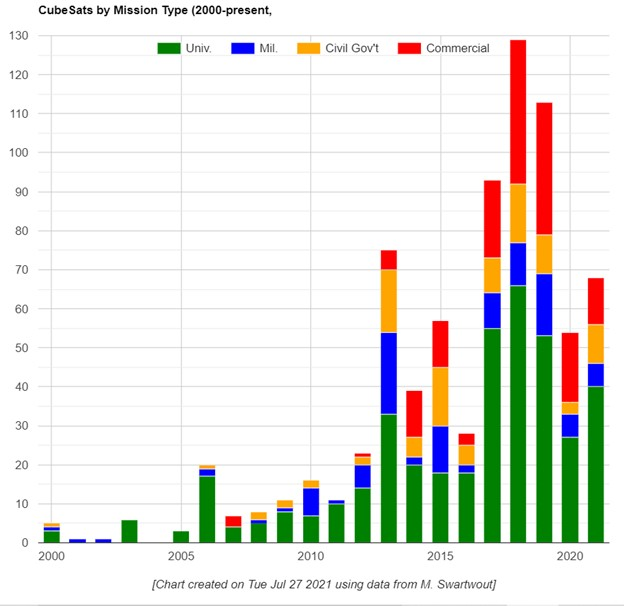
\includegraphics[width=.5\textwidth]{figure1}
    \caption{Nanosatellite launch data provided by M. Swartwout \cite:{2A}}
    \end{figure}
\section{CubeSats}

\subsection{What is SeaLion}
The SeaLion mission is a collaborative mission between Old Dominion University (ODU), the United Stated Coast Guard Academy (USCGA), and the Air Force Institute of Technology (AFIT) to design and produce a 3U CubeSat.

SeaLion consists of three payloads for on-orbit validation.  ODU provided one payload while the USCGA and AFIT provided the other two payloads.  SeaLion is planned to fly as a secondary payload on a Northrop Grumman Antares Rocket from Wallops Flight Facility (WFF), currently scheduled for March, 2023 \cite:{sealion_cdr}.  

\section{Model-Based Systems Engineering}
Traditional approaches use documents as their authoritative source of truth for conducting system engineering activities \cite:{architecting_spacecraft}.  However, these documents often do not have a living relationship with other documents or to other corresponding elements; thus, changes to one document require manual changes to other documents \cite:{ibm_mbse}.  Models provide the following key advantages over document-based approaches \cite:{ibm_mbse,value_and_benefits_mbse}:

\begin{enumerate}
\item Information is readily communicated and shared within the project

\item Changes are easily accommodated

\item Traceability is automated
\end{enumerate}

\subsection{Why Create a Modelling Language}

A common issue regarding tools for both students and amateur developers for system engineering is that many of the tools are proprietary and thus, unavailable to many potential users without significant cost burden \cite:{??}.  Thus, the goal of the Mach30 modeling language (m30ml), described herein, was to create an open-source tool that is readily available to anyone who wishes to model their respective systems while also making it easily learnable.  

\section{Mach30 Modelling Language}

The SeaLion Architecture uses m30ml to specify references, stakeholder needs, user stories, & data structures for facilitating traceability of design decisions within the Mission ConOps \cite:{mach30_git}.  The SeaLion repository is also structured as a Distributed OSHW Framework (DOF)-component for defining the contents of the Mission ConOps as a collection of nested subcomponents, component interfaces, and component functions for generating bill of materials (BOMs), assembly instructions, and/or usage documentation.

This is all done in an effort to execute the project via a documentation as code philosophy. A philosophy in which documentation is written with the same tools as code \cite:{docs_as_code}. This allows for workflows between development teams to be more closely integrated.

\end{document}

